\documentclass{standalone}
\usepackage{tikz, xcolor}
\usetikzlibrary{calc, quotes, arrows}
\usepackage{tikz-dimline}

\definecolor{tokushimaGold}{HTML}{fcd400}
\definecolor{tokushimaBlue}{HTML}{234794}

\begin{document}
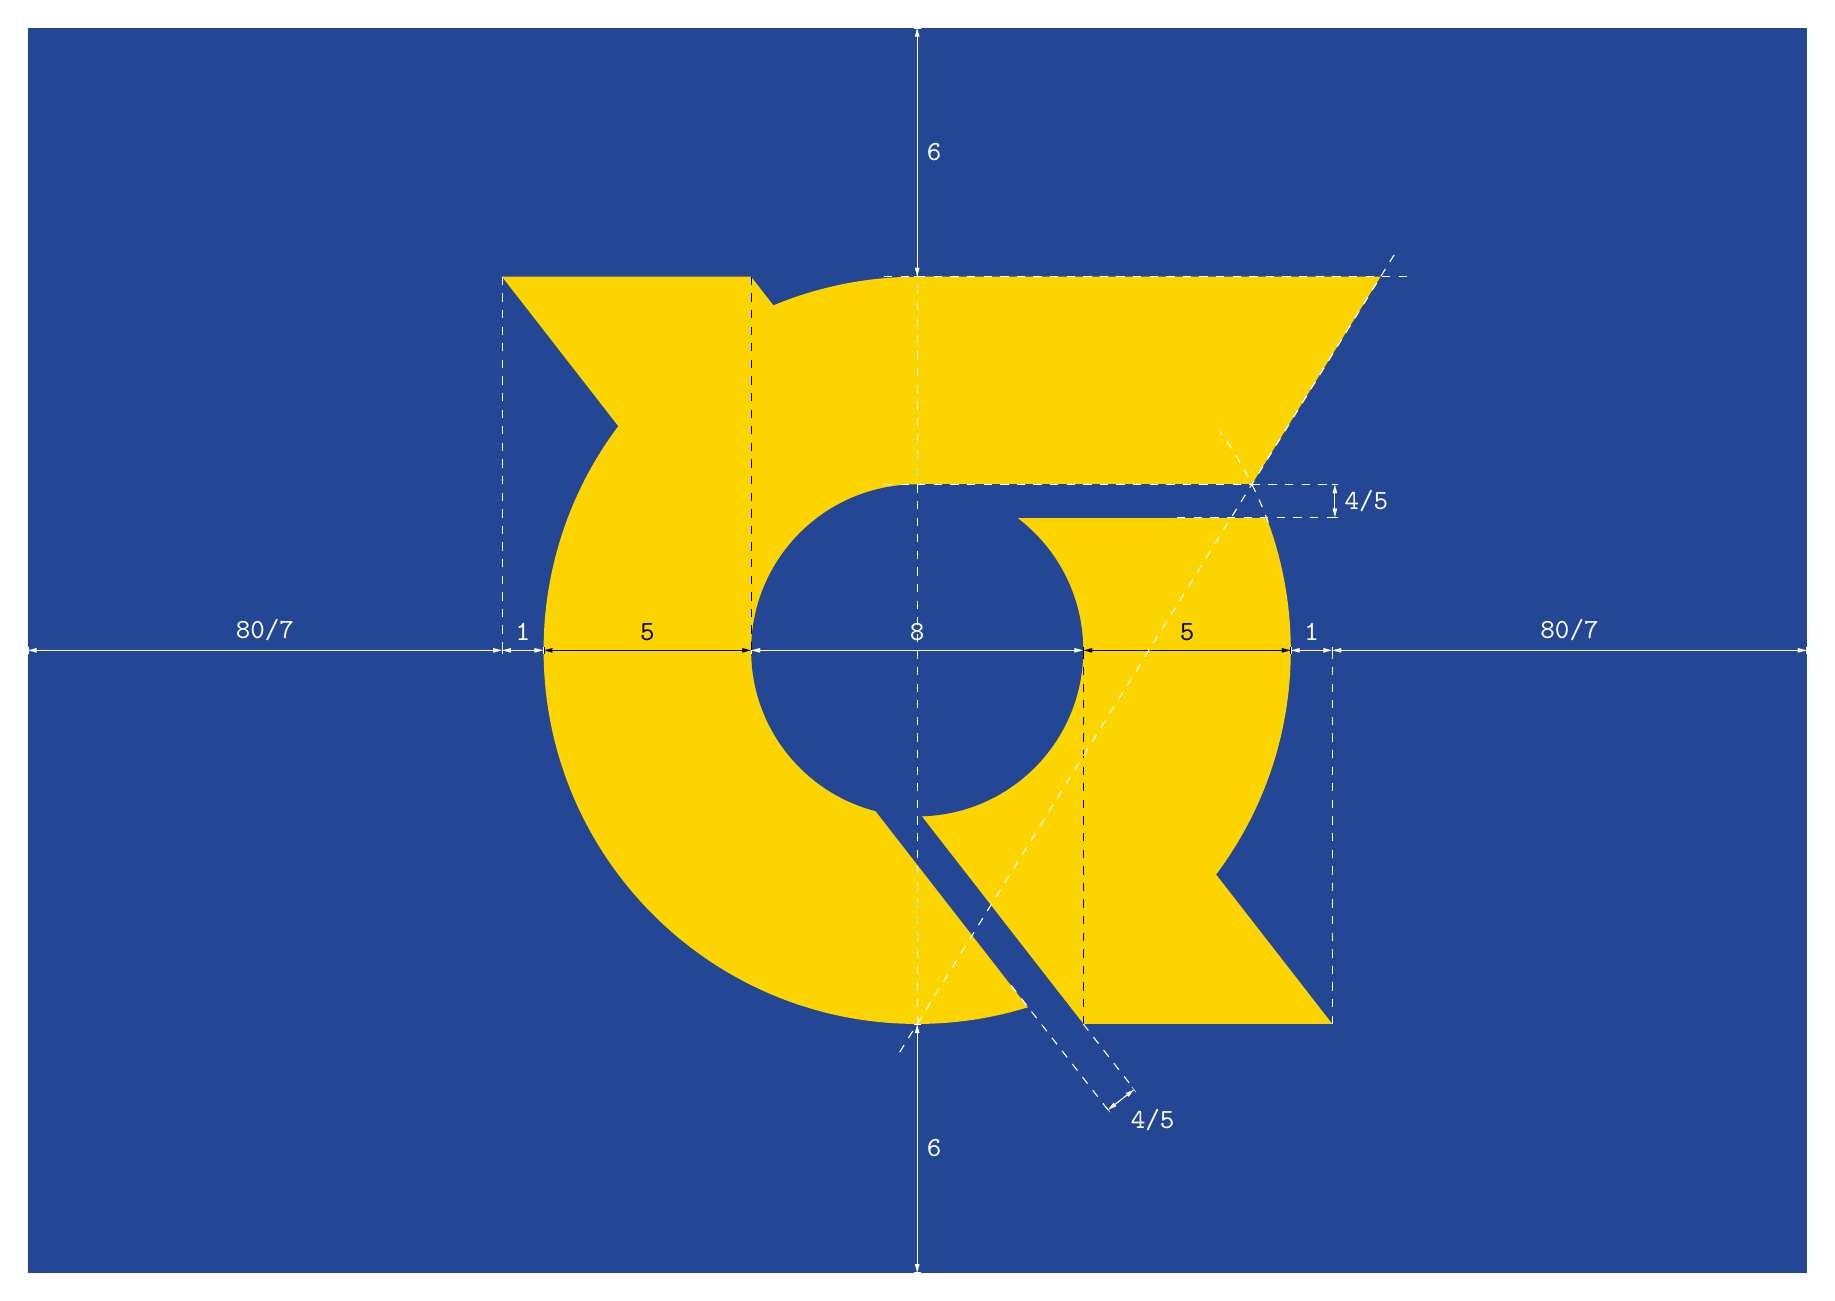
\begin{tikzpicture}[
        x=3pt,
        y=3pt,
        every node/.style={font=\ttfamily},
    ]
    \fill[use as bounding box, tokushimaBlue] (-900/4.2/2,-75) rectangle (900/4.2/2,75);
    \fill[tokushimaGold] (0,0) circle (45);
    \fill[tokushimaGold] (-50, 45) -- ++(30, 0) -- ++(70, -90) -- ++(-30, 0) -- cycle;
    \fill[tokushimaGold] (0, -45) -- ++(0, 90) -- ++(55.815630565, 0) -- cycle;
    \fill[tokushimaBlue] (0,0) circle (20);
    \fill[tokushimaBlue] (0, 20) -- ++(50,0) -- ++(0,-4) -- ++(-50,0) -- cycle;
    \fill[tokushimaBlue] (-1,-18) -- ++(21, -27) -- ++(-5.067446334, 0) -- ++(-21, 27) -- cycle;

    \path[
        dimline-dimline,
        every node/.style={font=\ttfamily},
    ]
    (-50, 0) edge["1",white] (-45, 0)
    (-45, 0) edge["5",black] (-20, 0)
    (-20, 0) edge["8",white] ( 20, 0)
    ( 20, 0) edge["5",black] ( 45, 0)
    ( 45, 0) edge["1",white] ( 50, 0)
    ( 0, 75) edge["6",white] ( 0, 45)
    ( 0,-45) edge["6",white] ( 0,-75)
    ( 50,0) edge["80/7",white] +(400/7,0)
    (-50,0) edge["80/7",white,swap] +(-400/7,0);
    \path[dashed]
    (-50, 0) edge[white] (-50, 45)
    (-20, 0) edge[black] (-20, 45)
    ( 20, 0) edge[black] ( 20,-45)
    ( 50, 0) edge[white] ( 50,-45);
    \path[
        dashed,
        white,
        shorten >=-12pt,
        shorten <=-12pt,
    ]
    ( 0,-45) edge (0, 45)
    ( 0, 45) edge (55.815630565,45)
    ( 0, 20) edge[shorten >=0] (55.815630565/90*65,20)
    ( 0,-45) edge (55.815630565,45);
    \draw[dashed, white]
    ([shift=(20:45)]0,0) arc  (20:36:45);

    \path
    (20,-45)                 coordinate (a1)
    ++({-atan(27/21)}:10)    coordinate (a2)
    ++({180+atan(21/27)}:4)  coordinate (a3)
    ++({180-atan(27/21)}:20) coordinate (a4);
    \path[white]
    (a1) edge[dashed] (a2)
    (a2) edge["4/5",dimline-dimline] (a3)
    (a3) edge[dashed] (a4);

    \path
    (55.815630565/90*65,20) coordinate (b1)
    ++(0:10)    coordinate (b2)
    ++(270:4)  coordinate (b3)
    ++(180:20) coordinate (b4);
    \path[white]
    (b1) edge[dashed] (b2)
    (b2) edge["4/5",dimline-dimline] (b3)
    (b3) edge[dashed] (b4);
\end{tikzpicture}

\end{document}
